% \newcommand{\prototitle}{Versuch 2 - Statistik}
% \newcommand{\Fachbereich}{Praktikum Messtechnik}
% \input{../packages/tu_header}

\newcommand{\institut}{Institut f\"ur Telekommunikationssysteme}
\newcommand{\fachgebiet}{Nachrichten\"ubertragung}
\newcommand{\veranstaltung}{Praktikum Nachrichten\"ubertragung}
\newcommand{\pdfautor}{\"Ozg\"u Dogan (326 048), Boris Henckell (325 779)}
\newcommand{\autor}{\"Ozg\"u Dogan (326 048)\\ Boris Henckell (325 779)}
\newcommand{\gruppe}{Gruppe: D03}
%\newcommand{\betreuer}{Betreuer: Mahmoud Felk}


\newcommand{\pdftitle}{Nachrichten\"ubertragung\ Praktikum\ 05}
\newcommand{\prototitle}{Praktikum 05 \\ HIER MUSS NOCH DER TITEL HIN}


\input{../../packages/tu_header_8}
% \begin{document}

% \lstlistoflistings
\definecolor{darkgray}{rgb}{0.95,0.95,0.95}
\definecolor{darkolivegreen}{HTML}{01a801}
\definecolor{functionsBlue}{HTML}{32b9b9}
\definecolor{variableRed}{rgb}{1,0,0}
\definecolor{stringBrown}{HTML}{bc8e8e} % f geht nicht

\lstset{
        %\lstset{extendedchars=true} % Umlaute an der richtigen stelle und nicht am Anfang ausgeben
        %basicstyle=\footnotesize\ttfamily,
        basicstyle=\small,
        %
        inputencoding=utf8,
        %
        tabsize=4,
        showspaces=false,
        showtabs=false,
        showstringspaces=true, % no special string spaces
        %
        backgroundcolor=\color{darkgray}, % background
        stringstyle=\color{stringBrown}\fseries, % Strings
        keywordstyle=\color{functionsBlue}\bfseries, % keywords Blau
        identifierstyle=\color{variableRed}, % variablen
        commentstyle=\color{darkolivegreen}, %  comments
        %
        breaklines=true,
        %
        numbers=left,
        numberstyle=\tiny,
        stepnumber=1,
        numbersep=7pt,
        %
        frame=single,
        columns=flexible,
        %
        xleftmargin=-2cm,
        xrightmargin=-1.5cm,
        %
        language=Matlab
}

%---------------------------------------------------------------------
%---------------------------------------------------------------------
%---------------------------------------------------------------------


\section{Einleitung}
\begin{quote}
	
	In diesem Termin wird eine Pulscodemodulation (PCM) Übertragungstrecke
	aufgebaut und untersucht. Außerdem wird der Ausmaß von Quantisierungsfehlern
	bei der digitalen Übertragung, sowie das Leistungsdichtespektrum (LDS) dieser
	Fehler gemessen.

\end{quote}%beende Einleitung
%--------------------------------------------------------------------
%--------------------------------------------------------------------    

\section{Motivation}
\begin{quote}
	
	Ursprünglich wurden Signale wie Mess-, Audio- und Bildsignale ausschließlich in
	analoger Form übertragen. Durch diese Art der Übertragung treten aber
	Rauschstörungen, lineare Verzerrungen (Änderungen des Frequenzganges) und
	nichtlineare Verzerrungen (Klirr) auf, welche auf der Empfängerseite kaum
	verringert werden können. Diese Störungen treten bei der digitalen Übertragung
	kaum auf, oder können beliebig klein gehalten werden, weshalb analoge Signale
	verstärkt anhand digitaler Kanäle übetragen werden.\\
	Eine Art der digitalen Übertragung ist die Pulscodemodulation.
	
\end{quote} %section

%--------------------------------------------------------------------
%--------------------------------------------------------------------    


\section{Theorie}
\begin{quote}

	Eine Pulscodemodulation basiert auf das Abtasten und Codeworterzeugung eines
	analogen Signals. Dabei wird das analoge Signal mithilfe eines A/D-Wandlers
	digitalisiert, codiert und nach der Übertragung beim Empfänger decodiert und
	mit einem D/A-Wandler wieder in ein analoges Signal umgewandelt. Eine
	Kanalcodierung des Übertragungskanal kann dabei für zusätzlichen Fehlerschutz
	vor Übertragungsfehlern sorgen.\\
	
	\begin{figure}[H]
    \centering
        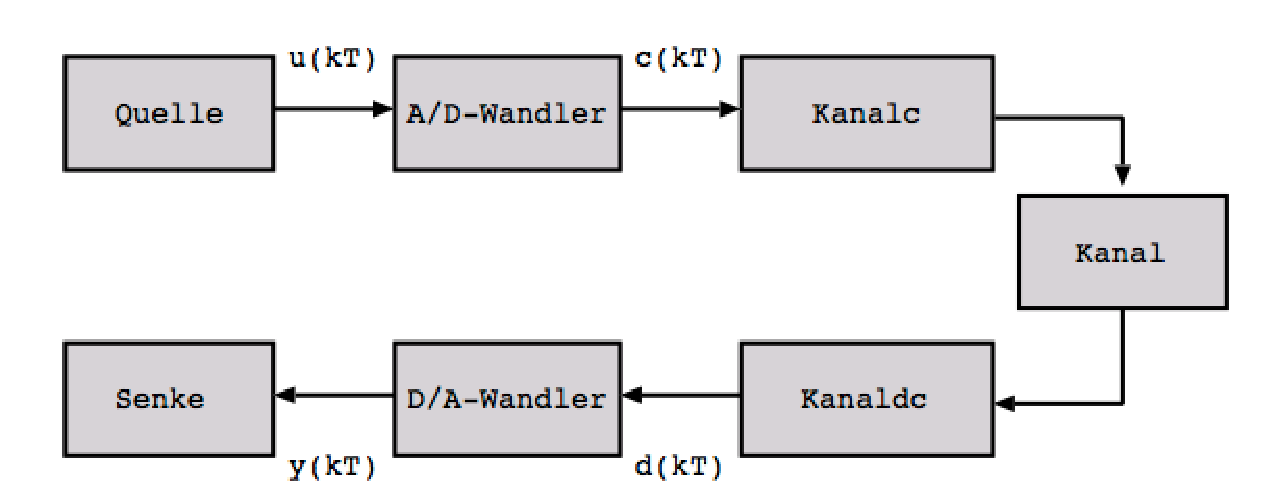
\includegraphics[scale=0.7, trim = 0cm 0cm 0cm 0cm, clip]{./Bilder/PCM-Uebertragung}
            \caption{PCM-Uebertragung}
            \cite{PCM-Uebertragung}
    \end{figure}
    
	
	Eine digitale Übertragung bietet viele Vorteile, wie zum Beispiel
	\begin{itemize}
		\item die Übertragungsqualität nimmt über weite Entfernungen durch den Einsatz
		von Regenerativverstärkern nicht ab
		\item die Multiplexbildung (z.B. TDM) ist vereinfacht
		\item es ist eine Integration von digitaler Übertragung und digitaler
		Vermittlung vorhanden
		\item die Wirtschaftlichkeit ist größer
		\item das Zusammenwirken mit digitalen Verfahren der Nachrichtenverarbeitung
		ist vereinfacht
		\item die Integration von Diensten ist möglich 
		\item es ist eine praktisch störungsfreie Übertragung durch Fehlerkorrekturen
		erreichbar
		\item und es besteht die Möglichkeit der Verschlüsselung um die Wahrung des
		Fernmeldegeheimnisses zu verbessern.
	\end{itemize}
	
	\vspace{1em}
	
	Die beiden Nachteile der digitalen Übertragung sind dagegen
	\begin{itemize}
		\item die Entstehung von Quantisierungfehlern
		\item und der erhöhte Bandbreitebedarf.
	\end{itemize}
	
	\vspace{0.5em}
	
	An dieser Stelle ist zu erwähnen, dass die Quantisierungfehler bei einer
	PCM-Übertragung relativ klein gehalten werden können und dass der höhere
	Bandbreitebedarf bei modernen digitalen verfahren mit effizienten
	Quellencodierungen und mehrstufigen Übertragungen der Binärinformation nicht
	mehr auftritt.\\
	
	\TODO{Frage: wo wurde das schon mal erwähnt?} \\
	Wie bereits erwähnt, wird bei der PCM-Übertragung das analoge Signal mit einer
	oberen Grenzfrequenz von $B_{Quelle}$ mit einer Abtastfrequenz von $f_T \geq 2
	\cdot B_{Quelle}$ abgetastet, wodurch ein PAM Signal mit den Abtastwerten im
	Abstand $T = \frac{1}{f_T}$ entsteht. Anhand eines Quantisierers wird diesen
	Werten jeweils eins von $M = 2^m$ möglichen wertdiskreten Signalen zugeordnet,
	deren Indizes in digitale Codewörter umgewandelt werden. Diese Codewörter sind
	typischerweise in binärer Form und bestehen aus $m = ld(M)$ Bit pro Abtastwert.
	Dabei einsteht eine Bitrate von
	
       \begin{equation*}
        	\begin{split}
        		R_{Bit} = f_T \cdot m \ \ \frac{bit}{s}
        	\end{split}
        \end{equation*}        
    
	\vspace{0.5em}
	   
	Zusammen ergeben der Abtaster, das Halteglied und der Quantisierer den
	A/D-Wandler bei der Digitalisierung eines analogen Signals.\\
	
	\begin{figure}[H]
    \centering
        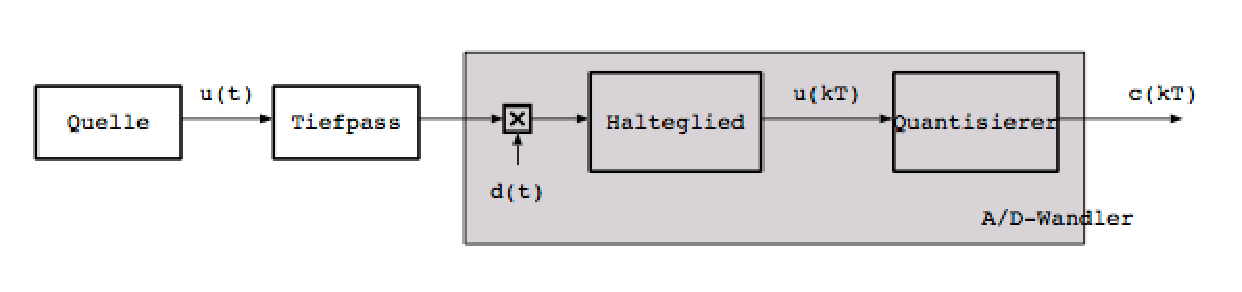
\includegraphics[scale=0.7, trim = 0cm 0cm 0cm 0cm, clip]{./Bilder/Digitalisierung_des_Signals}
            \caption{Blockschaltbild Digitalisierung eines Signals}
            \cite{Digitalisierung_des_Signals}
    \end{figure}
    
	
	Übertragen werden diese wertdiskreten Signale durch den digitalen Kanal, der
	sie bei fehlerfreier Übertragung eins zu eins an den Empfänger weitergibt. \TODO{was willst du mit dem nächsten satz
	sagen?} \\Dabei umfasst der Kanal von der Umwandlung in binäre Signalelemente über die
	Impulsformung und Modulation bishin zum Entscheider auf der Empfangsseite.\\
	Für die Kanalbandbreite bei einer binären Übertragung eines PCM-modulierten
	Signals und einer Bitrate von $R_{Bit} = f_T \cdot m \ \ \frac{bit}{s}$ gilt:
	 
       \begin{equation*}
        	\begin{split}
        		B_{Kanal,binäre PCM} = \frac{R}{2} \cdot (1+r)  =  m \cdot
        		B_{Quelle} \cdot (1+r)
        	\end{split}
        \end{equation*}        
        
	\vspace{0.5em}
	    
	Das $r$ entspricht dem Flankenfaktor, welcher einen Wert von $0 < r \leq 1$
	annehmen kann. Man sieht, dass für eine fehlerfreie Übertragung mindestens die
	 $m$-fache Quellbandbreite benötigt wird. Dieser kann aber wiederum verringert werden, wenn die $M$-wertigen
	Quantisierungsausgangswerte nicht in $m$ binäre Codewörter umgewandelt werden,
	sondern in $N$-wertige Codewörter. Dadurch entsteht in der Rechnung ein
	zusätzlicher Faktor, welcher die Kanalbandbreite reduziert:
	
	 \begin{equation*}
        	\begin{split}
        		B_{Kanal,N-wertige PCM} = \frac{m}{ld(N)} \cdot B_{Quelle} \cdot (1+r)
        	\end{split}
      \end{equation*}     
	
	\vspace{0.5em}
	
	Die Decodierung der übertragenen Codewörter erfolgt durch den Decodierer,
	welches aus einem D/A-Wandler und einem Rekonstruktionstiefpass besteht. Zuerst
	werden die empfangenen wertdiskreten Signale in $M$-wertige zeitdiskrete Abtastwerte
	umgewandelt, welche dann tiefpassgefiltert das ursprüngliche analoge Signal
	ergeben.\\
	
	\begin{figure}[H]
    \centering
        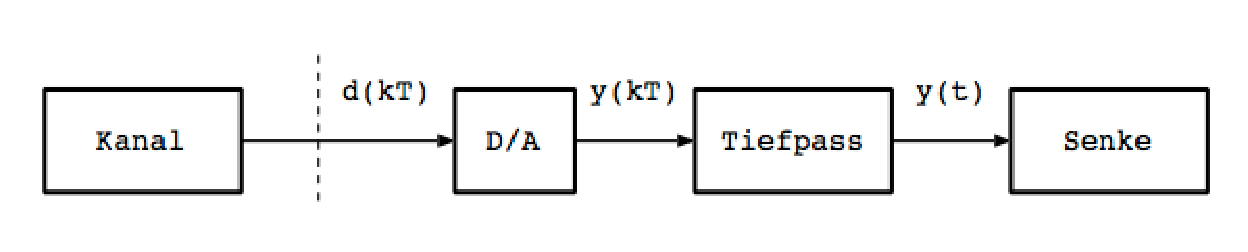
\includegraphics[scale=0.7, trim = 0cm 0cm 0cm 0cm, clip]{./Bilder/PCM_Decodierung}
            \caption{PCM Decodierung}
            \cite{PCM_Decodierung}
    \end{figure}
    
	
	Die PCM-Übertragung ist nur einer von vielen Verfahren der
	Digitalisierung, bei der eine Verringerung der notwendigen Bitrate möglich
	ist.Diese Übertragungsverfahren können mit dem Begriff Quellencodierung
	zusammengefasst werden und versichern keinen Qualitätsverlust. Um die besagte Bitrate zu verringern,
	werden die statistischen Eigenschaften der Nachrichtensignale und die
	Wahrnehmungseigenschaften der Menschen genutzt (Datenkompression).
	
	
	\end{quote}%section

%--------------------------------------------------------------------
%--------------------------------------------------------------------    
\section{Vorbereitungsaufgabe}
\begin{quote}
	
	Die theoretische Aufgabe für die Vorbereitung des Labortermin bestand darin,
	sich erneut mit dem Kapitel über Pulscodemodulation aus dem Skript zu
	beschäftigen. Das Wesentliche wurde in dem Theorieabschnitt des Protokolls
	erläutert. Außerdem sollten wir uns mit der Funktionsweise der für
	die PCM-Übertargungsstrecke relevanten Module des ETT-Schaltbretts vertraut
	machen und uns ein Blockschaltbild erarbeiten, welches den Aufbau realsieren
	könnte.\\
	
	\TODO{Blockschaltbild einfügen}
	
	Zuletzt sollte das in der Vorgabe gegebene MATLAB Skript PCM\_Analyse.m so
	vervollständigt werden, dass die Datei bei der Ausführung automatisch die
	PCM-Encoder-Kennlinie bestimmt. Der Code konnte anhand der Datei
	pcm\_data\_test.mat getestet und kontrolliert werden. 
	
	\TODO{Kennlinie einfügen und beschreiben}
	
\end{quote}%Theorie beenden

%--------------------------------------------------------------------
%--------------------------------------------------------------------    

    
\section{Labordurchführung}
\begin{quote}
         

         
\end{quote}%beende Labordurchführung

%--------------------------------------------------------------------
%--------------------------------------------------------------------    

    
\section{Auswertung}
\begin{quote}

         	
\end{quote}%beende Auswertung

%--------------------------------------------------------------------
%-------------------------------------------------------------------- 
    
\section{Zusammenfassung}
\begin{quote}


\end{quote}%beende Zusammenfassung
         

%--------------------------------------------------------------------
%--------------------------------------------------------------------    


\begin{thebibliography}{999}
 \bibitem {PCM-Uebertragung} Prof. Dr.-Ing. Sikora, Thomas; Prof. Dr.-Ing. Noll, Peter: Einführung in die
 Nachrichtenübertragung, S.272
\bibitem {Digitalisierung_des_Signals} Prof. Dr.-Ing. Sikora, Thomas; Prof. Dr.-Ing. Noll, Peter: Einführung in die
 Nachrichtenübertragung, S.273
\bibitem {PCM_Decodierung} Prof. Dr.-Ing. Sikora, Thomas; Prof. Dr.-Ing. Noll, Peter: Einführung in die
 Nachrichtenübertragung, S.276
 



%Name, Vorname.; evtl. Name2, Vorname2.: Titel des Dokumentes
%oder Buches, Zeitschrift/Verlag/URL (Auflage, Erscheinungsort, -jahr), ggf. Seitenzahlen
% \bibitem {PasevalscheTheorem} \url{https://de.wikipedia.org/wiki/Parsevalsches_Theorem}, Zugriff
% 23.05.2012
\end{thebibliography}

\end{document}
  	    
